\section{Observations}

\begin{table}[H]
\centering
\begin{tabular}{|c|c|c|} \hline
    $I$(A)& $2r$ (cm) & $r$ (cm)  \\ \hline
    1.333 & 12.2 & 6.10  \\
    1.436 & 10.9 & 5.45 \\
    1.542 & 10.1 & 5.05 \\
    1.634 &  9.7 & 4.85 \\
    1.736 &  9.0   & 4.50  \\
    1.840  &  8.5 & 4.25 \\
    1.943 &  8.1 & 4.05 \\
    2.041 &  7.7 & 3.85 \\
    2.142 &  7.2 & 3.60 \\
    2.239 &  6.9 & 3.45 \\
    2.320  &  6.7 & 3.35 \\
    2.449 &  6.3 & 3.15 \\
    2.613 &  6.0   & 3.00    \\
    2.720  &  5.7 & 2.85 \\
    2.817 &  5.6 & 2.80 \\
    \hline
    \end{tabular}    
    \caption{$I$ vs $r$ data for a fixed $U=300$ V}
    \label{tab:1}
\end{table}
\begin{table}[H]
    \centering
    \begin{tabular}{|c|c|c|}
    \hline
    $T$ (in $^\circ$C) & $V$ (mV) & $\rho$ ($\times 10^{-5}\,\Omega$ cm) \\ \hline
    32 & 0.044 & 7.806 \\ 
    40 & 0.045 & 7.984 \\ 
    43 & 0.046 & 8.161 \\ 
    46 & 0.047 & 8.338 \\ 
    49 & 0.050 & 8.871 \\ 
    64 & 0.055 & 9.758 \\ 
    67 & 0.057 & 10.113 \\ 
    74 & 0.059 & 10.467 \\ 
    75 & 0.060 & 10.645 \\ 
    78 & 0.061 & 10.822 \\ 
    84 & 0.062 & 11.000 \\ 
    89 & 0.063 & 11.177 \\ 
    90 & 0.064 & 11.355 \\ \hline
    \end{tabular}
    \caption{Temperature dependence of $V$ and subsequently $\rho$ of the Al sample at a fixed $I=100$ mA.}
\label{tab:2}
\end{table}
\begin{table}[H]
\centering
\begin{tabular}{|c|c|c|} \hline
    $U$ (V)& $2r$ (cm) & $r$ (cm)  \\ \hline
    299.9 & 7.8 & 3.90  \\
    290.4 & 7.7 & 3.85 \\
    279.1 & 7.6 & 3.80 \\
    270.2 & 7.4 & 3.70  \\
    260.3 & 7.3 & 3.65 \\
    250.7 & 7.0 & 3.50  \\
    240.5 & 6.8 & 3.40  \\
    230.6 & 6.7 & 3.35 \\
    219.9 & 6.5 & 3.25 \\
    210.8 & 6.4 & 3.20  \\
    200.2 & 6.3 & 3.15 \\
    \hline
    \end{tabular}    
    \caption{$U$ vs $r$ data for a fixed $I=2$ A}
    \label{tab:3}
\end{table}
\begin{table}[H]
\centering
\begin{tabular}{|c|c|c|} \hline
    $U$ (V)& $2r$ (cm) & $r$ (cm)  \\ \hline
    300.6 & 10.4 & 5.20  \\
    289.2 & 10.2 & 5.10  \\
    279.3 &  9.8 & 4.90  \\
    269.6 &  9.4 & 4.70  \\
    259.2 &  9.3 & 4.65 \\
    249.0   &  9.1 & 4.55 \\
    238.9 &  9.0   & 4.50  \\
    229.1 &  8.8 & 4.40  \\
    219.5 &  8.7 & 4.35 \\
    209.5 &  8.3 & 4.15 \\
    199.9 &  8.1 & 4.05 \\
    \hline
    \end{tabular}    
    \caption{$U$ vs $r$ data for a fixed $I=1.5$ A}
    \label{tab:4}
\end{table}

\section{Data Analysis and Calculations}

\subsection{For a Fixed Acceleration Potential}
    We can rearrange Eq. (8), to show,

    \begin{align}
        \frac{I^2}{1/r^2} &= \frac{2U}{(e/m_e)k^2} \nonumber\\
        \text{or, }\frac{e}{m_e} &= \frac{2U}{k^2\cdot m_1}
    \end{align}

    where $m_1$ is the slope of the $I^2$ vs $1/r^2$ plot.

    From table \ref{tab:1}, 

    \begin{figure}[H]
        \centering
        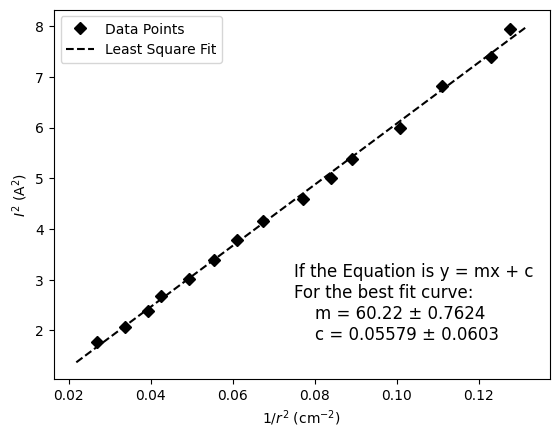
\includegraphics[height=0.7\columnwidth]{images/g1.png}
        \caption{$I^2$ vs $1/r^2$ plot for $U=300$ V}
        \label{graph:1}
    \end{figure}

    Here, $m_1=60.22$ A$^2$cm$^2$ and $U=300.0$ V. Hence using Eq. (9), specific charge of an electron, $e/m_e=1.641\cross10^{11}$ C kg$^{-1}$.

    Similarly, from table \ref{tab:2}, 

    \begin{figure}[H]
        \centering
        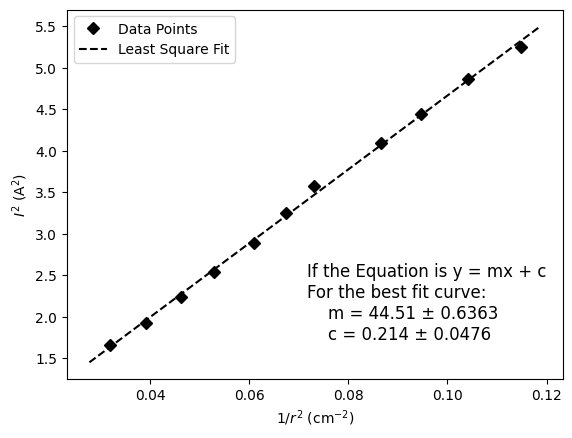
\includegraphics[height=0.7\columnwidth]{images/g2.png}
        \caption{$I^2$ vs $1/r^2$ plot for $U=249.7$ V}
        \label{graph:2}
    \end{figure}

    Here, $m_1=44.51$ A$^2$cm$^2$ and $U=249.7$ V. Hence using Eq. (9), specific charge of an electron, $e/m_e=1.847\cross10^{11}$ C kg$^{-1}$.

    Thus, the mean value of tthe specific charge of an electron, calculated using this method is $e/m_e=1.744\cross10^{11}$ C kg$^{-1}$.

\subsection{For a Fixed Current in the Helmholtz Coil}
    We can rearrange Eq. (8), to show,

    \begin{align}
        \frac{r^2}{U} &= \frac{2}{(e/m_e)k^2I^2} \nonumber\\
        \text{or, }\frac{e}{m_e} &= \frac{2m_2}{k^2I^2}
    \end{align}

    where $m_2$ is the slope of the $U$ vs $r^2$ plot.

    From table \ref{tab:3}, 

    \begin{figure}[H]
        \centering
        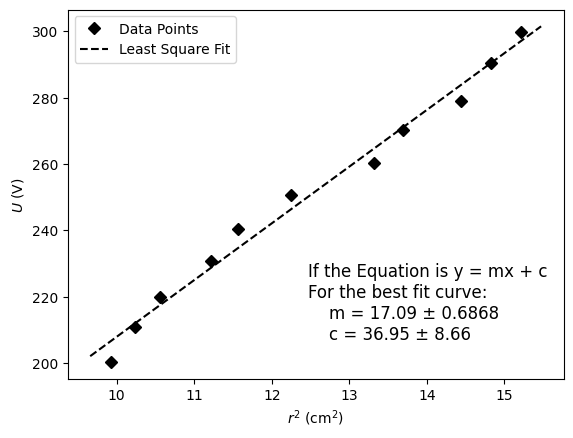
\includegraphics[height=0.7\columnwidth]{images/g3.png}
        \caption{$U$ vs $r^2$ plot for $I=2.0$ A}
        \label{graph:3}
    \end{figure}

    Here, $m_2=17.09$ V cm$^{-2}$ and $I=2.0$ A. Hence using Eq. (10), specific charge of an electron, $e/m_e=1.408\cross10^{11}$ C kg$^{-1}$.

    Similarly, from table \ref{tab:4}, 

    \begin{figure}[H]
        \centering
        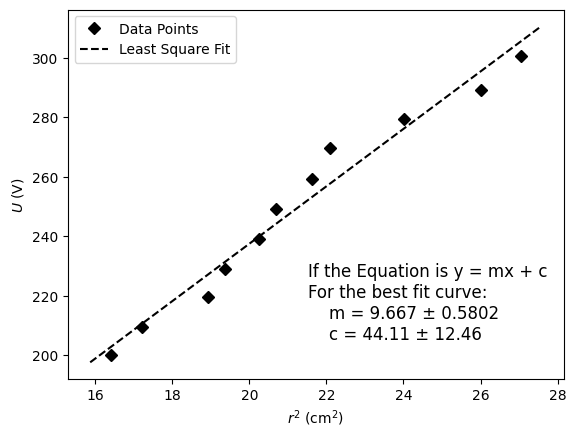
\includegraphics[height=0.7\columnwidth]{images/g4.png}
        \caption{$U$ vs $r^2$ plot for $I=1.5$ A}
        \label{graph:4}
    \end{figure}

    Here, $m_2=9.667$ V cm$^{-2}$ and $I=1.5$ A. Hence using Eq. (10), specific charge of an electron, $e/m_e=1.411\cross10^{11}$ C kg$^{-1}$.

    Thus, the mean value of the specific charge of an electron, calculated using this method is $e/m_e=1.410\cross10^{11}$ C kg$^{-1}$.